\newif\ifen
\newif\ifes
\newcommand{\en}[1]{\ifen#1\fi}
\newcommand{\es}[1]{\ifes#1\fi}
\entrue
\usepackage[utf8]{inputenc}
\documentclass[a0,portrait]{a0poster} %A0 841mm x 1189mm
\usepackage{multicol} % This is so we can have multiple columns 
\columnsep=80pt % This is the amount of white space between the columns in the poster
\columnseprule=3pt % This is the thickness of the black line between the columns in the poster

\usepackage[svgnames]{xcolor} % Specify colors by their 'svgnames', for a full list of all colors available see here: http://www.latextemplates.com/svgnames-colors
\usepackage[makeroom]{cancel} % \cancel{} \bcancel{} etc
\usepackage{multirow}
%\usepackage{times} % Use the times font
%\usepackage{palatino} % Uncomment to use the Palatino font
%\usepackage[sfdefault]{AlegreyaSans}
\usepackage[sfdefault]{AlegreyaSans}

\usepackage{graphicx} % Required for including images
\graphicspath{{figures/}} % Location of the graphics files
\usepackage{booktabs} % Top and bottom rules for table
\usepackage[labelfont=bf]{caption} % Required for specifying captions to tables and figures
\captionsetup[subfigure]{font=Large}
\captionsetup[figure]{font=Large}
\usepackage{amsfonts, amsmath, amsthm, amssymb} % For math fonts, symbols and environments
\usepackage{wrapfig} % Allows wrapping text around tables and figures
\usepackage{bm}
\usepackage{ragged2e}
\usepackage{float} % para que los gr\'aficos se queden en su lugar con [H]
\usepackage[subrefformat=parens]{subcaption} % para \begin{subfigure}
\usepackage{tikz} % Para graficar, por ejemplo bayes networks
\usepackage{framed}
\usepackage{mdframed}
  
\usepackage[absolute,overlay]{textpos} 
\setlength{\TPHorizModule}{1cm} %
\setlength{\TPVertModule}{1cm}	%

\newcommand{\E}{\en{S}\es{E}}
\newcommand{\A}{\en{E}\es{A}}
\newcommand{\Ee}{\en{s}\es{e}}
\newcommand{\Aa}{\en{e}\es{a}}


\usetikzlibrary{bayesnet} % Para que ande se necesita copiar el archivo  tikzlibrarybayesnet.code.tex en la misma carpeta


\newcommand{\vm}[1]{\mathbf{#1}}
\newcommand{\N}{\mathcal{N}}
\newcommand\hfrac[2]{\genfrac{}{}{0pt}{}{#1}{#2}} %\frac{}{} sin la linea del medio

% \usepackage{xr}
% \externaldocument{supplementary}
\setlength{\columnseprule}{0pt}


\addtolength{\textwidth}{40pt}
\addtolength{\oddsidemargin}{-40pt}
 
\begin{document}
% 
% \begin{textblock}{100}(18,23.25)
%  \includegraphics[width=0.1\textwidth]{auxliar/images/dc_color.pdf} 
%  \end{textblock}
% \begin{textblock}{100}(30,24)
%  \includegraphics[width=0.1\textwidth]{auxliar/images/icc-logo.jpg} 
%  \end{textblock}
%  \begin{textblock}{100}(49,24)
%  \includegraphics[width=0.1\textwidth]{auxliar/images/logo_licar.pdf} 
%  \end{textblock}
%   \begin{textblock}{100}(61,24)
%  \includegraphics[width=0.1\textwidth]{auxliar/images/logo_version_02.pdf} 
%  \end{textblock}
%  
%----------------------------------------------------------------------------------------
%	POSTER HEADER 
%----------------------------------------------------------------------------------------

% The header is divided into two boxes:
% The first is 75% wide and houses the title, subtitle, names, university/organization and contact information
% The second is 25% wide and houses a logo for your university/organization or a photo of you
% The widths of these boxes can be easily edited to accommodate your content as you see fit
\centering \fontsize{90}{90} \textbf{Bayesian inference: learning and  evolution} \\[0.4cm]  % Title
\fontsize{70}{85}\textbf{}\\[1cm] % Subtitle
\LARGE \textbf{Gustavo Landfried}  \ \ \  \texttt{glandfried@dc.uba.ar} \\
\large 1. Universidad de Buenos Aires. Facultad de Ciencias Exactas y Naturales. Departamento de Computaci\'on. Buenos Aires, Argentina \\ 
\large 2. CONICET-Universidad de Buenos Aires. Instituto de Investigaci\'on en Ciencias de la Computaci\'on (ICC). Buenos Aires, Argentina \\


 % A bit of extra whitespace between the header and poster content
\vspace{1cm}
%----------------------------------------------------------------------------------------


%\begin{paracol}{2}
\begin{multicols}{2}
% This is how many columns your poster will be broken into, a portrait poster is generally split into 2 columns
\fontsize{40}{50}\selectfont






















\centrering

{\fontsize{60}{72}\selectfont \textbf{TrueSkill Through Time (TTT)} \\[0.2cm]
\LARGE \textbf{Reliable initial skill estimates and historical comparability} } \\[0.8cm]

\justify 


\en{Unlike the most commonly used skill estimators in the video game industry (Elo, TrueSkill, Glicko), the TTT model obtains reliable initial skill estimates and guarantees historical comparability by propagating the whole information in a single Bayesian network. }%
\es{A diferencia de los estimadores de habilidad más utilizados en la industria del video juego (e.g Elo, TrueSkill, Glicko), el modelo TTT obtiene estimaciones fiables de la habilidad inicial y garantiza la comparabilidad histórica gracias a que propaga toda la información histórica en una única red bayesiana. }%
%
\en{In this paper we offer the first package for \texttt{Julia}, \texttt{Python} and \texttt{R}, a high-performance algorithm that allows millions of observations to be analyzed using any low-end computer. }%
\es{En este artículo ofrecemos el primer paquete para \texttt{Julia}, \texttt{Python} y \texttt{R}, un algoritmo de alto desempeño que permite analizar millones de observaciones usando cualquier ordenador de gama baja. }

\vspace{1.5cm}

\textbf{Introduc\en{tion}\es{ción}.} HOla
\begin{figure}[H]
\begin{subfigure}[c]{0.49\linewidth}
  \centering
  \scalebox{1.25}{
      \tikz{         
    \node[det, fill=black!10] (r) {$r$} ; 
    \node[inv, below=of r] (ir) {} ; 
    \node[const, left=of r, xshift=-1.35cm] (r_name) {\small \en{Result}\es{Resultado}:}; 
    \node[const, right=of r] (dr) {$ r = (d > 0)$}; 

    \node[latent, above=of r, yshift=-1cm] (d) {$d$} ; %
    \node[const, right=of d] (dd) {$ d = p_i-p_j$}; 
    \node[const, left=of d, xshift=-1.35cm] (d_name) {\small \en{Difference}\es{Diferencia}:};
    
    \node[latent, above=of d, xshift=-1.5cm, yshift=-1cm] (p1) {$p_i$} ; %
    \node[latent, above=of d, xshift=1.5cm, yshift=-1cm] (p2) {$p_j$} ; %
    \node[const, left=of p1, xshift=-0.25cm] (p_name) {\small \en{Performance}\es{Desempeño}:}; 

    \node[accion, above=of p1,yshift=0.5cm] (s1) {} ; %
    \node[const, right=of s1] (ds1) {$s_i$};
    \node[accion, above=of p2,yshift=0.5cm] (s2) {} ; %
    \node[const, right=of s2] (ds2) {$s_j$};
    
    
%     \node[latent, above=of p1,yshift=-1cm] (s1) {$s_i$} ; %
%     \node[latent, above=of p2,yshift=-1cm] (s2) {$s_j$} ; %
%     
%     \node[const, right=of p2] (dp2) { $p \sim \N(s,\beta^2)$};
%     \node[const, right=of s2] (ds2) { $s \sim \N(\mu,\sigma^2)$}; 
%     
    
    \node[const, right=of p2] (dp2) { $p \sim \N(s,\beta^2)$};

    \node[const, left=of s1, xshift=-.85cm] (s_name) {\small \en{Skill}\es{Habilidad}:}; 
    
    \edge {d} {r};
    \edge {p1,p2} {d};
    \edge {s1} {p1};
    \edge {s2} {p2};
    
 }
  }
  \end{subfigure}
  \begin{subfigure}[c]{0.49\linewidth}
  \centering
    \en{\includegraphics[page={1},width=\linewidth]{figures/posterior_win}}
    \es{\includegraphics[page={2},width=\linewidth]{figures/posterior_win}}
  \end{subfigure}
\end{figure}


\begin{figure}[H]
  \centering
  \scalebox{1.5}{
    \tikz{ %
      \node[latent] (s10) {$s_{a_0}$} ;
      %
      \node[latent,  below=of s10,yshift=-0.7cm] (s11) {$s_{a_1}$} ;
      
      \node[latent, right=of s11, xshift=-1cm] (p11) {$p_{a_1}$} ;
      %
      \node[latent, below=of s11,yshift=-0.4cm] (s12) {$s_{a_2}$} ;
      \node[latent, right=of s12, xshift=-1cm] (p12) {$p_{a_2}$} ;
      
      \node[const, right=of p11,xshift=0.4cm] (r1) {$\bm{>}$} ;
      \node[const, above=of r1, yshift=0.5cm] (nr1) {\footnotesize \ \  Observed result} ;
      \node[const, right=of p12,xshift=0.4cm] (r2) {$\bm{<}$} ;
      \node[const, above=of r2, yshift=0.5cm] (nr2) {\footnotesize \ \ Observed result} ;
      
      \node[latent, left=of s10, xshift=11.4cm] (s20) {$s_{b_0}$} ;
      \node[latent, below=of s20,yshift=-0.7cm] (s21) {$s_{b_1}$} ;
      \node[latent, left=of s21, xshift=1cm] (p21) {$p_{b_1}$} ;
      
      \node[latent, below=of s21, yshift=-0.4cm] (s22) {$s_{b_2}$} ;
      \node[latent, left=of s22, xshift=1cm] (p22) {$p_{b_2}$} ;
      
      
      \edge {s10} {s11};
      \edge {s11} {s12};
      \edge {s20} {s21};
      \edge {s21} {s22};
      \edge {s11} {p11};
      \edge {s12} {p12};
      \edge {s21} {p21};
      \edge {s22} {p22};
      
      \node[const, left=of s10, yshift=0.5cm ] (wp10) {\includegraphics[page={13},width=.175\linewidth]{figures/smoothing}} ;
      \node[const, right=of s20, yshift=0.5cm ] (wp20) {\includegraphics[page={13},width=.175\linewidth]{figures/smoothing}} ;
      
      
      \node[const, left=of s11, yshift=0.6cm ] (post11) {\includegraphics[page={1},width=.175\linewidth]{figures/smoothing}} ;
      %\node[const, right=of s11, yshift=0.6cm ] (wp11) {\includegraphics[page={2},width=.125\linewidth]{figures/smoothing}} ;
      %\node[const, left=of p11, yshift=0.6cm ] (lh11) {\includegraphics[page={3},width=.125\linewidth]{figures/smoothing}} ;
      
      \node[const, left=of s12, yshift=0.6cm ] (post12) {\includegraphics[page={4},width=.175\linewidth]{figures/smoothing}} ;
      %\node[const, right=of s12, yshift=0.6cm ] (wp12) {\includegraphics[page={5},width=.125\linewidth]{figures/smoothing}} ;
      %\node[const, left=of p12, yshift=0.6cm ] (lh12) {\includegraphics[page={6},width=.125\linewidth]{figures/smoothing}} ;
      
      
      \node[const, right=of s21, yshift=0.6cm ] (post21) {\includegraphics[page={7},width=.175\linewidth]{figures/smoothing}} ;
      %\node[const, left=of s21, yshift=0.6cm ] (wp21) {\includegraphics[page={8},width=.125\linewidth]{figures/smoothing}} ;
      %\node[const, right=of p21, yshift=0.6cm ] (lh21) {\includegraphics[page={9},width=.125\linewidth]{figures/smoothing}} ;
      
      
      \node[const, right=of s22, yshift=0.6cm ] (post22) {\includegraphics[page={10},width=.175\linewidth]{figures/smoothing}} ;
      %\node[const, left=of s22, yshift=0.6cm ] (wp22) {\includegraphics[page={11},width=.125\linewidth]{figures/smoothing}} ;
      %\node[const, right=of p22, yshift=0.6cm ] (lh22) {\includegraphics[page={12},width=.125\linewidth]{figures/smoothing}} ;
      
      }  
  }
\end{figure}


% \begin{equation*}
%  P(\text{Model\es{o}}|\text{Dat\en{a}\es{os}}) = \frac{P(\text{Dat\en{a}\es{os}}|\text{Model\es{o}})P(\text{Model\es{o}})}{P(\text{Dat\en{a}\es{os}})}
% \end{equation*}

\begin{equation}\label{eq:bayes_factor}
 \frac{P(\text{Model\es{o}}_i|\text{Dat\en{a}\es{os}})}{P(\text{Model\es{o}}_j|\text{Dat\en{a}\es{os}})} = \frac{P(\text{Dat\en{a}\es{os}}|\text{Model\es{o}}_i)\cancel{P(\text{Model\es{o}}_i)}}{P(\text{Dat\en{a}\es{os}}|\text{Model\es{o}}_j)\cancel{P(\text{Model\es{o}}_j)}}% \overset{\text{\en{if}\es{si} } *}{=} \frac{P(\text{Dat\en{a}\es{os}}|\text{Model\es{o}}_i)}{P(\text{Dat\en{a}\es{os}}|\text{Model\es{o}}_j)} 
\end{equation}
%
with
\begin{equation*}
\begin{split}
P(\text{Dat\en{a}\es{os}}|\text{Model\es{o}}) & = P(d_1|\text{Model\es{o}})P(d_2|d_1,\text{Model\es{o}}) \dots \\
& = \text{geometric mean}(P(\text{Dat\en{a}\es{os}}|\text{Model\es{o}}))^{|\text{Dat\en{a}\es{os}}|}
\end{split}
\end{equation*}


% \begin{figure}[H]
% \centering
% \scalebox{1.33}{
% \tikz{
%     \node[const] (a1) {\includegraphics[page=1,width=0.2\linewidth]{figures/trueskillthroughtime}};
%     \node[const, left=of a1] (na) {\en{Player}\es{Jugador} A:};
%     \node[const,right=of a1] (a2) {\includegraphics[page=2,width=0.2\linewidth]{figures/trueskillthroughtime}}; 
%     \node[const,below=of a1] (b1) {\includegraphics[page=3,width=0.2\linewidth]{figures/trueskillthroughtime}}; 
%     \node[const, left=of b1] (nb) {\en{Player}\es{Jugador} B:};
%     \node[const,below=of a2] (b2) {\includegraphics[page=4,width=0.2\linewidth]{figures/trueskillthroughtime}}; 
%     \node[const, above=of a1] (g1) {Game 1 ($p_A > p_B$)};
%     \node[const, above=of a2] (g2) {Game 2 ($p_A < p_B$)};
%     
% }
% }
% \caption{
%  \en{Estimates obtained with TrueSkill (red) and with TrueSkill Through Time (green) after having seen two players compete twice: the first time player A wins and the second time player B wins. }%
%  \es{Estimaciones obtenidos con TrueSkill (rojo) y con TrueSkill Through Time (verde) luego de haber visto a dos jugadores competir dos veces: la primera gana el jugador A y en la segunda el jugador B. }%
% }
% \label{fig:trueskillthroughtime}
% \end{figure}

%
\begin{table}[H] \centering
  \begin{tabular}{c|cc|cc|cc|cc|c||c} 
 \multirow{2}{*}{$\hfrac{\text{\scriptsize Dataset}}{\text{Test size}}$} & \multicolumn{2}{c|}{Constant\es{e}$^\dagger$}& \multicolumn{2}{c|}{Elo$^\dagger$} & \multicolumn{2}{c|}{TrueSkill} & \multicolumn{2}{c|}{KickScore$^\dagger$} &  \multicolumn{2}{c}{TTT} \\
 & GM & $\log_2$BF & GM & $\log_2$BF & GM & $\log_2$BF & GM & $\log_2$BF & GM & LOOCV \\ \hline
\multirow{2}{*}{$\hfrac{\text{\scriptsize Ten\en{n}is}}{\num{186361}}$} & \multirow{2}{*}{$0.5593$} & \multirow{2}{*}{\num{7910}} & \multirow{2}{*}{$0.5695$} & \multirow{2}{*}{\num{3051}} & \multirow{2}{*}{$0.5722$} & \multirow{2}{*}{\num{1780}} & \multirow{2}{*}{$0.5758$} & \multirow{2}{*}{\num{93}} & \multirow{2}{*}{$\bm{0.5760}$} & \multirow{2}{*}{${0.5908}$} \\
 & & & & & & & & & & \\
 \multirow{2}{*}{$\hfrac{\text{\scriptsize Basketball}}{\num{20300}}$} & \multirow{2}{*}{$0.5006$} & \multirow{2}{*}{\num{1771}} & \multirow{2}{*}{$0.5305$} & \multirow{2}{*}{\num{72}} & \multirow{2}{*}{$0.5316$} & \multirow{2}{*}{\num{11}} & \multirow{2}{*}{$\bm{0.5328}$} & \multirow{2}{*}{-55} & \multirow{2}{*}{${0.5318}$} & \multirow{2}{*}{${0.5382}$} \\
  & & & & & & & & & & \\
 \multirow{2}{*}{$\hfrac{\text{\scriptsize Chess}}{\num{92004}}$} & \multirow{2}{*}{$0.3570$} & \multirow{2}{*}{\num{520}} & \multirow{2}{*}{$0.3552$} & \multirow{2}{*}{\num{1190}} & \multirow{2}{*}{$0.3580$} & \multirow{2}{*}{\num{148}} & \multirow{2}{*}{$\bm{0.3584}$} & \multirow{2}{*}{0} & \multirow{2}{*}{$\bm{0.3584}$} & \multirow{2}{*}{${0.3641}$} \\
 & & & & & & & & & \\
 \multirow{2}{*}{$\hfrac{\text{\scriptsize \en{Football}\es{Fútbol}}}{\num{5759}}$} & \multirow{2}{*}{$0.3949$} & \multirow{2}{*}{\num{30}} & \multirow{2}{*}{$0.3867$} & \multirow{2}{*}{\num{204}} & \multirow{2}{*}{$0.3921$} & \multirow{2}{*}{\num{89}} & \multirow{2}{*}{$\bm{0.3961}$} & \multirow{2}{*}{\num{4}} & \multirow{2}{*}{$\bm{0.3963}$} &  \multirow{2}{*}{${0.3974}$} \\
  & & & & & & & & & & \\ \hline
  \end{tabular}
%   \caption{
%   \en{Comparisons between different models in four databases. }%
%   \es{Comparaciones entre los modelos TTT, KickScore, TrueSkill, Elo y Constant en cuatro base de datos. }%
%   %
%   \en{The GM columns report the geometric mean of the a priori predictions of the models, Eq.~\eqref{eq:gmean}. }%
%   \es{Las columnas GM reportan la media geométrica de las predicciones a priori de los modelos (ecuación \ref{eq:gmean}). }%
%   %
%   \en{The $\log_2$BF columns report the Bayes Factor, Eq.~\eqref{eq:bayes_factor}, between TTT and the other models in the logarithmic scale. }%
%   \es{Las columnas $\text{log}_2$BF reportan el Bayes Factor (ecuación \ref{eq:bayes_factor}) entre TTT y otros modelos en escala logarítmica. }%
%   %
%   \en{For reference, the LOOCV column reports the geometric mean of the predictions using all historical data, $p(d_i| d_1, \dots, d_{i-1}, d_{i+1}, \dots, d_n , M)$. }%
%   \es{Como referencia, la columna LOOCV reporta la media geométrica de las predicciones usando toda la información histórica, $p(d_i| d_1, \dots, d_{i-1}, d_{i+1}, \dots, d_n , M)$. }%
%   %
%   \en{The geometric mean of the models marked with the symbol $\dagger$ was computed by \cite{Maystre2019}. }%
%   \es{La media geométrica de los modelos señalados con el símbolo $\dagger$ fue obtenida por \cite{Maystre2019}. }%
%   }
%   \label{Tab:Models}
\end{table}


\begin{figure}[H]
% \centering
\begin{subfigure}[b]{1\linewidth}
    \centering
    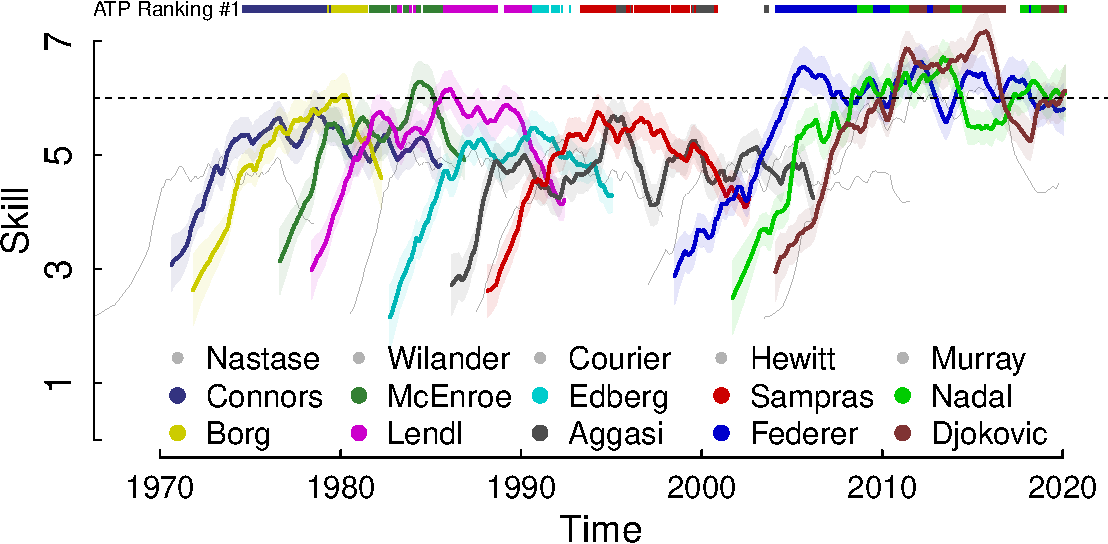
\includegraphics[width=.99\linewidth]{static/atp}
    \caption{
    \en{Estimated learning curves for some famous male players. }%
    \es{Curvas de aprendizaje estimadas de algunos jugadores masculinos. }%
    }
    \label{fig:atp}
\end{subfigure}
\end{figure}


\columnbreak


























\centering

{\fontsize{60}{72}\selectfont \textbf{Evolutionary - Probabilistic isomorphism} \\[0.2cm]
\LARGE \textbf{The irreversible emergence of cooperation and specialization} } \\[0.8cm]

\justify

\en{The current complexity of life is the consequence of a series of evolutionary transitions in which entities capable of self-replication after the transition become part of higher level cooperative units (eukaryotic cells, multicellular organisms, social systems). }%~\cite{maynardSmith1995-majorTransitions, szathmary1995-evolutionaryTransitions, szathmary2015-evolutionaryTransitions}
\es{La complejidad actual de la vida es consecuencia de una serie de transiciones evolutivas en las que entidades capaces de autoreplicación luego de la transición pasan a formar parte de unidades cooperativas de nivel superior (células eucariotas, organismos multicelululares (células eucariotas, organismos multicelulares, sistemas sociales). }%~\cite{maynardSmith1995-majorTransitions, szathmary1995-evolutionaryTransitions, szathmary2015-evolutionaryTransitions}
%
\en{In this paper we show that the advantage in favor of cooperation and specialization is so common in the history of life because of the multiplicative nature of evolutionary and probabilistic selection processes. }%
\es{En este trabajo mostramos que la ventaja a favor de la cooperación y la especialización es tan común en la historia de la vida debido a la naturaleza multiplicativa de los procesos de selección evolutiva y probabilística. }%

\vspace{1.5cm}

% 
% \begin{figure}[H]
% \centering
%  \begin{subfigure}[b]{1\linewidth}    
%  \centering
%  \scalebox{1.6}{
%  \tikz{
%         
%     \node[obs] (a1) {$\vec{\A}^{\,1}$};
%     \node[obs, right=of a1] (a2) {$\vec{\A}^{\,2}$};
%     \node[const, left=of a1] (na) {\text{\en{Environment}\es{Ambiente}:\,}};
%     
%     \node[const, above=of a1, xshift=0cm, yshift=0.3cm] (pa) {$P(\Aa) = p^\Aa (1-p)^{1-\Aa}$};
%     
%     \node[latent, below=of a1 ] (i1) {$I^1$};
%     \node[latent, below=of a2 ] (i2) {$I^2$};
%     \node[latent, right=of i2 ] (i3) {$I^3$};
%     \node[const, left=of i1] (ni) {\text{\en{Individuals}\es{Individuos}:\,}};
%     
%     \node[const, above=of a2,  xshift=7cm, yshift=0.3cm] (pie) {$P(i|\vec{\Aa}) \propto \Ee_i^{\Aa_i} (1-\Ee_i)^{1-\Aa_i}$};
%     
%     \node[const, above=of i3] (pii) {$P(i^{t+1}|i^t) = 
% \begin{cases}
% 1/N & \texttt{coop}(i^t) \wedge (\texttt{reg}(i^{t+1}) = \texttt{reg}(i^{t})) \\
% 1 & \neg \texttt{coop}(i^t) \wedge i^{t+1} = i^t \\
% 0 & \texttt{else} \\
% \end{cases}$};
%     
%     \node[latent, below=of i1 ] (c1) {$G^1$};
%     \node[latent, below=of i2 ] (c2) {$G^2$};
%     \node[latent , below=of i3 ] (c3) {$G^3$};
%     \node[const, left=of c1] (nc) {\text{\en{Groups}\es{Grupos}:\,}};
%     
%     \node[invisible, below=of c2, yshift=-0.5cm] (inv) {};
%     
%     
%     \edge {a1} {i1};
%     \edge {a2} {i2};
%     \edge {i1} {i2,c1};
%     \edge {i2} {i3,c2};
%     \edge {i3} {c3};
%     
%     }}
%  \end{subfigure}
% \end{figure}
%  
% \begin{equation}\tag{isomorphism}
% \text{Bayes' theorem} \equiv \text{Replicator dynamic}
% \end{equation}

\textbf{Introduc\en{tion}\es{ción}}
\en{The evolutionary growth of a lineage over time, $\omega(t)$, is governed by a sequence of survival and reproduction rates $f(\cdot)$ }%
\es{El crecimiento evolutivo de un linaje en el tiempo, $\omega(t)$, esta gobernado por una secuencias estocástica de tasas de supervivencia y reproducción $f(\cdot)$ }%
%
\begin{equation} \label{eq:modelo_exponencial}
\omega(T) = \prod_t^T f(\Aa(t)) \approx g^T \ \ \text{ with } \ \ f(\Aa) =
\begin{cases}
 1.5 & \Aa = \text{ \en{Head}\es{Cara} } \\
 0.6 & \Aa = \text{ \en{Tail}\es{Sello} }
\end{cases}
\end{equation}
%
\en{According to the \emph{replicator dynamic} equation \cite{taylor1978-replicatorDynamic}, the proportion of a strategy in the population, $P(\Ee|\Aa^1 \dots \Aa ^T)$, is determined by }%
\es{Según el modelo estándar de evolución, conocido como \emph{replicator dynamic} \cite{taylor1978-replicatorDynamic}, la proporción de una estrategia en la población, $P(\Ee|\Aa^1 \dots \Aa ^T)$, está determinado por }%
% schuster1983-replicatorDynamics, hofbauer2003-evolutionaryGameDynamics
%
\begin{equation} \label{eq:replicator_dynamic}  \tag{Isomorphism}
P(\Ee|\Aa^1 \dots \Aa ^T) = \frac{P(\Ee|\Aa^1 \dots \Aa ^{T-1}) f(\Ee,\Aa)}{\sum_s P(\Ee|\Aa^1 \dots \Aa ^{T-1}) f(\Ee,\Aa)}
\end{equation}
%
\en{Which is the characteristic growth rate $g$? }%
\es{¿Cuál es la tasa de crecimiento característica $g$? }%

\vspace{0.3cm}

\begin{figure}[H]
    \centering
    \begin{subfigure}[b]{0.49\linewidth}
    \includegraphics[width=\linewidth]{figures/pdf/ergodicity_expectedValue.pdf}
    \caption*{Arithmetic: $1.5 \cdot \frac{1}{2} + 0.6 \cdot  \frac{1}{2} = 1.05$}
    \end{subfigure}
    \begin{subfigure}[b]{0.49\linewidth}
    \includegraphics[width=\linewidth]{figures/pdf/ergodicity_individual_trayectories.pdf}
    \caption*{Geometric: $(1.5 \cdot 0.6)^{1/2} \approx 0.95$}
    \end{subfigure}
\end{figure}

\textbf{Result\en{s}\es{ados}}

\en{Cooperation reduces fluctuations and increases the growth rate. }%
\es{La cooperación reduce las fluctuaciones y aumenta la tasa de crecimiento. }%
%
\en{Defection increases fluctuations and reduces the growth rate. }%
\es{La desercion aumenta las fluctuaciones y reduce la tasa de crecimiento. }%
%
\begin{figure}[H]
    \centering
    \begin{subfigure}[b]{0.5\linewidth}
    \includegraphics[width=\linewidth]{figures/pdf/ergodicity_desertion.pdf}
    \end{subfigure}
\end{figure}

\en{As soon as cooperation emerges, an advantage in favor of specialist strategies appears. }%
\es{Apenas surge la cooperación, aparece una ventaja a favor de las estrategias especialistas. }%

\begin{figure}[H]
    \centering
    \begin{subfigure}[b]{0.49\linewidth}
    \includegraphics[width=\linewidth]{figures/pdf/tasa-temporal-0.pdf}
    \end{subfigure}
    \begin{subfigure}[b]{0.49\linewidth}
    \includegraphics[width=\linewidth]{figures/pdf/tasa-temporal-2.pdf}
    \end{subfigure}
    \label{fig:tasa-temporal-2}
\end{figure}

\en{Since specialist strategies are individually poorly adapted to the environment, an irreversibility of the evolutionary transition is created. }%
\es{Como la estrategias especialistas están individualmente mal adaptadas al ambiente, se crea una irreversbilidad de la transiciones evolutivas. }%

\vspace{0.5cm}

\textbf{Conclution.} The advantage in favor of cooperation and specialization is due to the multiplicative nature of evolutionary and probabilistic selection processes.





\end{multicols}
{ \footnotesize
%\nocite{*} % Print all references regardless of whether they were cited in the poster or not
\bibliographystyle{./biblio/plos2015} % Plain referencing style
\bibliography{./biblio/biblio.bib} % Use the example bibliography file sample.bib
}
\end{document}
